\graphicspath{{./chapter2/}}

\section{Chapter 2: Multi-arm Bandits}
RL evaluates the actions taken rather than instructs correct actions like other forms of learning.
\subsection{An \(n\)-Armed Bandit Problem}
\textbf{The problem}

\begin{itemize}
\item You are faced repeatedly with a choice of n actions.

\item After each choice, you receive a reward from a \textbf{stationary} probability distribution (reward for an action is sampled from the same prob dist every time). 

\item Objective is to maximise total reward over some time period, say 100 time steps.

\item Named after of slot machine (one-armed bandit problem), but \(n\) levers instead of 1.

\item Each action has an expected or mean reward based on its probability distribution. We
shall call this the \textbf{value} of the action. We do not know these values with certainty.
Because of this uncertainty, there is always an \textbf{exploration} vs \textbf{exploitation} problem. We
always have one action that we deem to be most valuable at any instant, but it is highly
likely, at least initially, that there are actions we are yet to explore that are more valuable.

\end{itemize}





%-------------------------------------- SUBSECTION -----------------------------------------------

\subsection{Action-Value Methods}
The estimated action value is

\begin{equation}
Q_t(a) \doteq \frac{
    \text{sum of rewards when $a$ was taken prior to $t$}
}{
    \text{number of times $a$ was taken prior to $t$}
} = \frac{
\sum_{i=1}^{t-1} R_i \cdot \mathbbm{1}_{A_i = a}
}{
\sum_{i=1}^{t-1} \mathbbm{1}_{A_i = a}
},
\tag{2.1}
\end{equation}

where $\mathbbm{1}_{\textit{predicate}}$ denotes the random variable that is 1 if \textit{predicate} is true and 0 if it is not.  

If the denominator is zero, then we instead define $Q_t(a)$ as some default value, such as 0. As the denominator goes to infinity, by the law of large numbers, $Q_t(a)$ converges to $q_*(a)$.  


\begin{equation}
\LARGE Q_t(a) \xrightarrow[t \to \inf]{} q_*(a)
\label{eq:sample_average_convergence}
\end{equation}

Call this the \textit{sample-average} method for estimating action values because each
estimate is an average of the sample of observed rewards.


The true value (mean reward) of an action is \(q\), but the \textit{estimated} value at the \(t\)-th time-step
is \(Q_t(a)\)

The \textbf{greedy} action selection method is
\begin{equation}
A_t = \arg\max_a Q_t(a)
\tag{2.2}
\end{equation}

\begin{itemize}
\item Simplest action selection rule is to select the action with the highest estimated value. 
\item $\epsilon$-greedy methods are where the agent selects the greedy option most of the time, and selects a random action with probability $\epsilon$.
\item Three algorithms are tried: one with \(e\)=0 (pure greedy), one with \(e\)=0.01 and another with \(e\)=0.1
\item Greedy method gets stuck performing sub-optimal actions.
\item e=0.1 explores more and usually finds the optimal action earlier, but never selects it more at 91\% of the time.
\item e=0.01 method improves more slowly, but eventually performs better than the \(e\)=0.1 on both performance measures.
\item It is possible to reduce \(e\) over time to try to get the best of both high and low values.
\end{itemize}

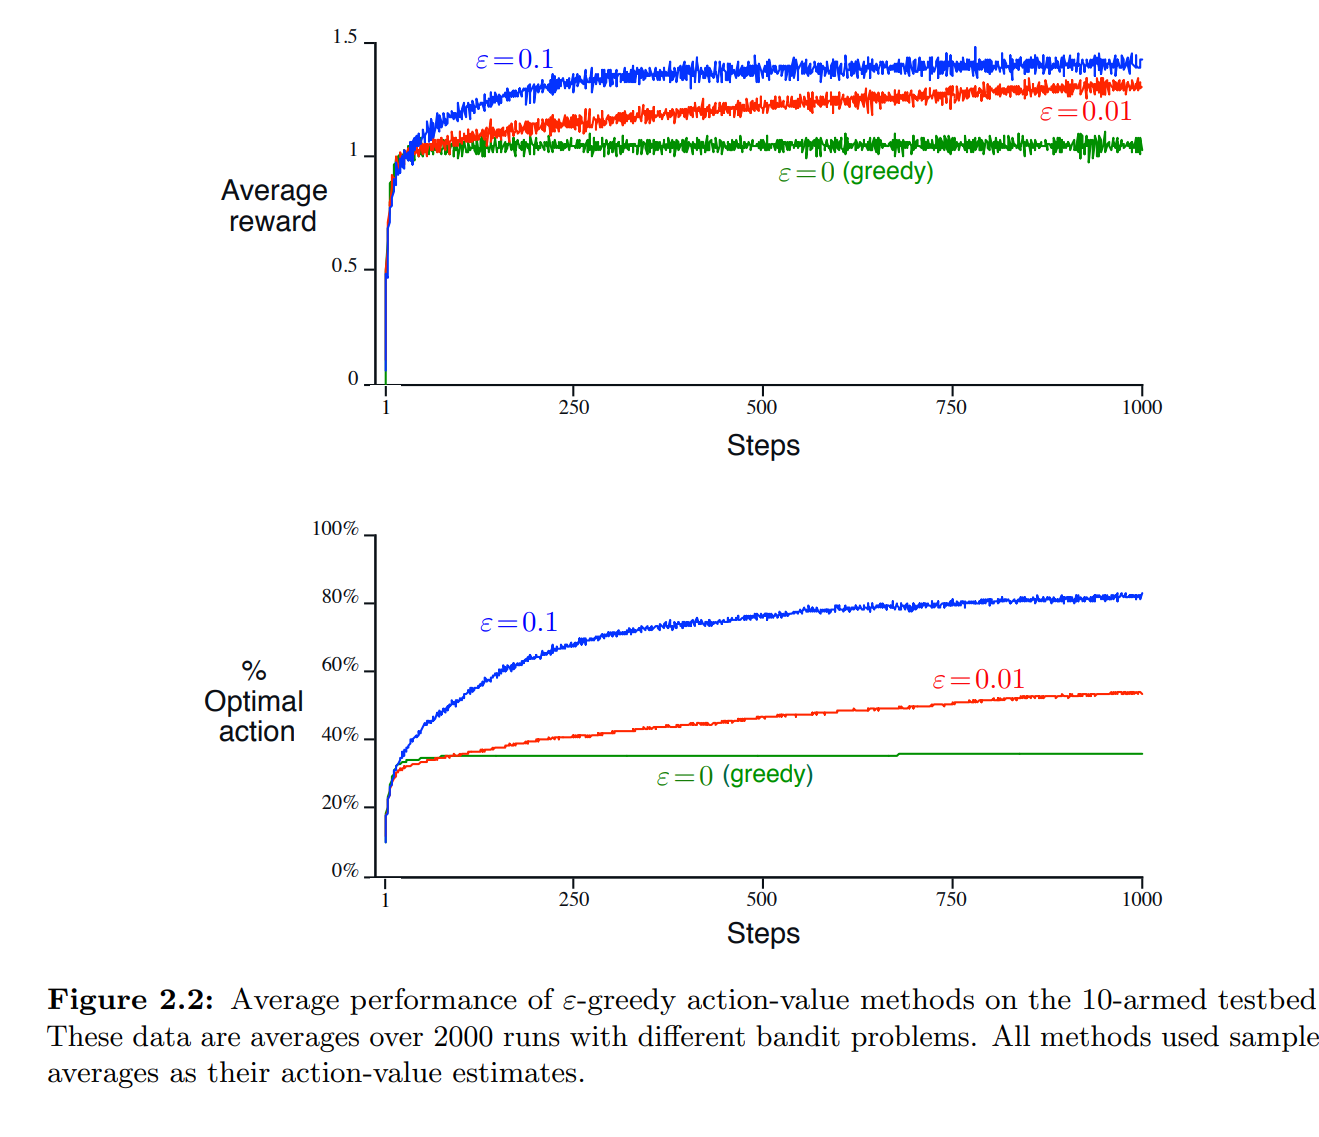
\includegraphics[scale=0.3]{./greedy_action_value_graph.png}


\subsubsection{Exercises}
\QuestionAnswer{
Bandit example Consider a \(k\)-armed bandit problem with \(k = 4\) actions,
denoted 1, 2, 3, and 4. Consider applying to this problem a bandit algorithm using
$\epsilon$-greedy action selection, sample-average action-value estimates, and initial estimates
of \(Q_1(a) = 0\), for all \(a\). Suppose the initial sequence of actions and rewards is \(A_1 = 1,
R_1 = -1, A_2 = 2, R_2 = 1, A_3 = 2, R_3 = -2, A_4 = 2, R_4 = 2, A_5 = 3, R_5 = 0\). On some
of these time steps the " case may have occurred, causing an action to be selected at
random. On which time steps did this definitely occur? On which time steps could this
possibly have occurred?
}
{
\begin{enumerate}
\item At \(t = 1\), we have \(Q_1(1) = 0\), \(Q_1(2) = 0\), \(Q_1(3) = 0\), and \(Q_1(4) = 0\). Any choice here could be greedy or exploration, so exploration \textit{could have} occured. 1 is selected, and the action value for 1 is updated to \(Q_2(1) = \frac{R_1}{1} = \frac{-1}{1} = -1\).
\item At \(t = 2\), we have \(Q_2(1) = -1\), \(Q_2(2) = 0\), \(Q_2(3) = 0\), and \(Q_2(4) = 0\). Any choice but 1 here could be greedy or exploration, so exploration \textit{could have} occured. The action value for 2 is updated to \(Q_3(2) = 1\).
\item At \(t = 3\), we have \(Q_3(1) = -1\), \(Q_3(2) = 1\), \(Q_3(3) = 0\), and \(Q_3(4) = 0\). 2 is selected again, and the action value for 2 is updated to \(Q_4(2) = \frac{1 + (-2)}{2} = \frac{-1}{2} = -0.5\).
\item At \(t = 4\), we have \(Q_4(1) = -1\), \(Q_4(2) = -0.5\), \(Q_4(3) = 0\), and \(Q_4(4) = 0\). 2 is selected again even though its value is \(0 < Q_4(3) \text{ and } 0 < Q_4(4) \). So, \textit{definitely} exploration.  the action value for 2 is updated to \(Q_5(2) = \frac{-1 + 2}{3} = \frac{1}{3} = 0.33\).
\item At \(t = 5\), we have \(Q_5(1) = -1\), \(Q_5(2) = 0.33\), \(Q_5(3) = 0\), and \(Q_5(4) = 0\). 3 is selected even though its value is \(0 < Q_5(2)\) = 0.33. Therefore, we \textit{definitely} explored here. 
\end{enumerate}

\begin{table}[H]
\centering
\begin{tabular}{|c|l|l|l|}
\hline
\textbf{Time \(t\)} & \textbf{Action Values \(Q_t(a)\)} & \textbf{Action Chosen} & \textbf{Exploration?} \\
\hline
1 &
\(Q_1(a) = 0\) for all \(a\) &
\(A_1 = 1\) &
Possibly (all values tied) \\
\hline
2 &
\(
\begin{aligned}
Q_2(1) &= -1 \\
Q_2(2) &= 0 \\
Q_2(3) &= 0 \\
Q_2(4) &= 0
\end{aligned}
\) &
\(A_2 = 2\) &
Possibly (multiple actions tied for max) \\
\hline
3 &
\(
\begin{aligned}
Q_3(1) &= -1 \\
Q_3(2) &= 1 \\
Q_3(3) &= 0 \\
Q_3(4) &= 0
\end{aligned}
\) &
\(A_3 = 2\) &
Definitely greedy (2 is best) \\
\hline
4 &
\(
\begin{aligned}
Q_4(1) &= -1 \\
Q_4(2) &= -0.5 \\
Q_4(3) &= 0 \\
Q_4(4) &= 0
\end{aligned}
\) &
\(A_4 = 2\) &
Definitely exploration (2 is suboptimal) \\
\hline
5 &
\(
\begin{aligned}
Q_5(1) &= -1 \\
Q_5(2) &= 0.33 \\
Q_5(3) &= 0 \\
Q_5(4) &= 0
\end{aligned}
\) &
\(A_5 = 3\) &
Definitely exploration (3 < 2) \\
\hline
\end{tabular}
\caption{Analysis of exploration vs. greedy choices using \(\epsilon\)-greedy algorithm.}
\end{table}
}

\QuestionAnswer{
    In the comparison shown in Figure 2.2, which method will perform best in
the long run in terms of cumulative reward and probability of selecting the best action?
How much better will it be? Express your answer quantitatively
}
{
According to Equation \ref{eq:sample_average_convergence}, the method with $\epsilon$ = 0.01 will choose the optimal action 10x more often than the one with $\epsilon$=0.1 because 
as \(t \rightarrow \infty\), all \(Q_{\infty}(a) \rightarrow q_*(a)\).
}





% --------------------------------------------------- SUBSECTION -------------------------------------------------------------------

\subsection{Incremental Implementation}
The sample-average technique used to estimate action-values above has a problem: memory and computation requirements grow over time. This isn't necessary, we can devise an incremental solution instead:
\begin{align}
Q_{k+1} &= \frac{1}{k} \sum_{i=1}^{k} R_i \\
&= \frac{1}{k} \left( R_k + \sum_{i=1}^{k-1} R_i \right) \\
&\vdots \nonumber \\
&= Q_k + \frac{1}{k} [R_k - Q_k]
\end{align}
We are updating our estimate of $Q_{k+1}$ by adding the discounted error between the reward just received and our estimate for that reward $Q_k$.
\begin{equation}
\textit{NewEstimate} \leftarrow \textit{OldEstimate} + \textit{StepSize} [\textit{Target} - \textit{OldEstimate}]
\label{eq:incremental_update}
\end{equation}
$\alpha$ is used to denote the stepsize ($\frac{1}{k}$) in the rest of this book.





% -------------------------------------------------- SUBSECTION ---------------------------------------------------------------------

\subsection{Non-Stationary Problems}

Most problems in RL are \textbf{non-stationary} - the reward for an action is sampled from a prob dist that changes over time.

$\Rightarrow$ Give more weight to recent rewards, since their rewards are sampled from the most recent prob dists.

For example, the incremental update rule in Equation (\ref{eq:incremental_update}) for updating an average $Q_n$ of the $n-1$ past rewards is modified to be
\begin{equation}
Q_{n+1} \doteq Q_n + \alpha [R_n - Q_n] , 
\end{equation}
where the step-size parameter $\alpha \in (0, 1]$ is \textbf{constant}. This results in $Q_{n+1}$ being a weighted average of past rewards and the initial estimate $Q_1$:
\begin{align}
Q_{n+1} &= Q_n + \alpha [R_n - Q_n] \nonumber \\
&= \alpha R_n + (1-\alpha)Q_n \nonumber \\
&= \alpha R_n + (1-\alpha)[\alpha R_{n-1} + (1-\alpha)Q_{n-1}] \nonumber \\
&= \alpha R_n + (1-\alpha)\alpha R_{n-1} + (1-\alpha)^2 Q_{n-1} \nonumber \\
&= \alpha R_n + (1-\alpha)\alpha R_{n-1} + (1-\alpha)^2 \alpha R_{n-2} + \dots \nonumber \\
& \qquad \dots + (1-\alpha)^{n-1} \alpha R_1 + (1-\alpha)^n Q_1 \nonumber \\
&= (1-\alpha)^n Q_1 + \sum_{i=1}^{n} \alpha (1-\alpha)^{n-i} R_i . 
\label{eq:constant_stepsize_update}
\end{align}


\begin{itemize}
\item Call this the \textbf{constant-stepsize} method for estimating action values.
\item The sum of the weights add up to 1. 
\item Since $\alpha \in (0, 1]$, the weight given to \(R_i\) decreases exponentially. We call this method \textit{exponential recency-weighted average}.
\end{itemize}






% ------------------------------------------------------ SUBSECTION ------------------------------------------------
\subsection{Optimistic Initial Values}
\begin{itemize}
\item The methods discussed so far are dependent to some extent on the initial action-value
    estimate i.e. they are biased by their initial estimates.
\item For methods with constant $\alpha$ this bias is permanent.
\item In effect, the initial estimates become a set of parameters for the model that must be
    picked by the user.
\item In the above problem, by initial bias to +5 rather than 0 we encourage exploration, even in the greedy case. The agent will almost always be disappointed with it's
    samples because they are less than the initial estimate and so will explore elsewhere until
    the values converge.
\item The above method of exploration is called \textit{Optimistic Initial Values}
\item ONLY suited for \textbf{stationary} problems. NOT suited for \textbf{non-stationary} problems since the drive for exploratory is only temporary.
\end{itemize}

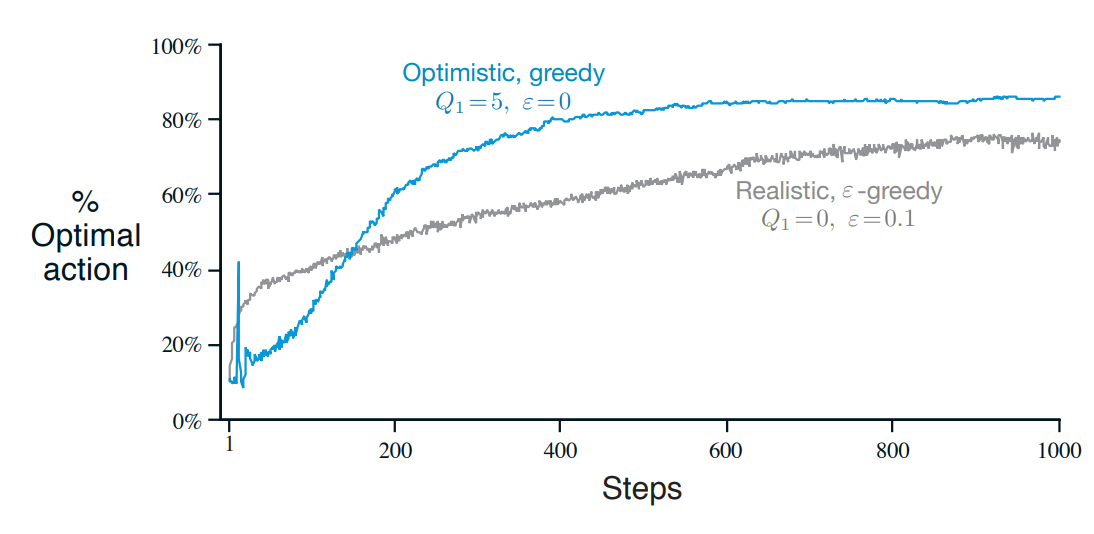
\includegraphics[scale=0.35]{./optimistic_initial_value_graph.png}


\subsubsection{Exercises}
\QuestionAnswer{
Mysterious Spikes The results shown in Figure 2.3 should be quite reliable
because they are averages over 2000 individual, randomly chosen 10-armed bandit tasks.
Why, then, are there oscillations and spikes in the early part of the curve for the optimistic
method? In other words, what might make this method perform particularly better or
worse, on average, on particular early steps?
}
{
The spikes could happen because the model initially selected the optimistic action, but then its reward was almost always less than the large initial bias, so 
the model was disappointed and explored other actions. 
}

\QuestionAnswer{

}{

We are given the update rule for the $n$-th reward for a particular action:
$Q_n \leftarrow Q_{n-1} + \beta_n [R_n - Q_{n-1}]$, where $Q_0$ is the initial estimate.
This can be written as:
\begin{equation}
Q_n = (1-\beta_n)Q_{n-1} + \beta_n R_n \quad (*)
\end{equation}

The step size $\beta_n$ is defined as:
\begin{equation}
\beta_n = \alpha / \bar{o}_n \quad (\text{cf. Eq. 2.8 in source})
\end{equation}
where $\alpha > 0$ is a constant step size, and $\bar{o}_n$ is a trace updated by:
\begin{equation}
\bar{o}_n = \bar{o}_{n-1} + \alpha(1 - \bar{o}_{n-1}) = (1-\alpha)\bar{o}_{n-1} + \alpha, \quad \text{for } n > 0, \text{ with } \bar{o}_0 = 0 \quad (\text{cf. Eq. 2.9 in source}).
\end{equation}

{\large Analyze $\bar{o}_n$}

The recurrence for $\bar{o}_n$ is $\bar{o}_n = (1-\alpha)\bar{o}_{n-1} + \alpha$.
We can find a closed form for $\bar{o}_n$. Let $\bar{o}_n = 1 - \delta_n$.
\begin{align*}
1 - \delta_n &= (1-\alpha)(1 - \delta_{n-1}) + \alpha \\
1 - \delta_n &= 1 - \delta_{n-1} - \alpha + \alpha\delta_{n-1} + \alpha \\
1 - \delta_n &= 1 - (1-\alpha)\delta_{n-1}
\end{align*}
So, $\delta_n = (1-\alpha)\delta_{n-1}$.
Given $\bar{o}_0 = 0$, we have $1-\delta_0 = 0 \implies \delta_0 = 1$.
Thus, $\delta_n = (1-\alpha)^n \delta_0 = (1-\alpha)^n$.
Therefore,
\begin{equation}
\bar{o}_n = 1 - (1-\alpha)^n.
\end{equation}

{\large Substitute $\beta_n$ into the update rule for $Q_n$}

From $Q_n = (1-\beta_n)Q_{n-1} + \beta_n R_n$:
Using $\beta_n = \alpha / \bar{o}_n$:
\begin{align*}
Q_n &= \left(1 - \frac{\alpha}{\bar{o}_n}\right)Q_{n-1} + \frac{\alpha}{\bar{o}_n} R_n \\
\bar{o}_n Q_n &= (\bar{o}_n - \alpha)Q_{n-1} + \alpha R_n.
\end{align*}
We know $\bar{o}_n = (1-\alpha)\bar{o}_{n-1} + \alpha$, so $\bar{o}_n - \alpha = (1-\alpha)\bar{o}_{n-1}$.
Substituting this into the equation for $\bar{o}_n Q_n$:
\begin{equation}
\bar{o}_n Q_n = (1-\alpha)\bar{o}_{n-1}Q_{n-1} + \alpha R_n.
\end{equation}

{\large Expand the recurrence for $\bar{o}_n Q_n$}

Let $X_n = \bar{o}_n Q_n$. The recurrence is $X_n = (1-\alpha)X_{n-1} + \alpha R_n$.
This is a standard first-order linear recurrence relation. We can expand it:
\begin{align*}
X_n &= (1-\alpha)X_{n-1} + \alpha R_n \\
X_n &= (1-\alpha)((1-\alpha)X_{n-2} + \alpha R_{n-1}) + \alpha R_n \\
X_n &= (1-\alpha)^2 X_{n-2} + (1-\alpha)\alpha R_{n-1} + \alpha R_n \\
&\vdotswithin{=} \\
X_n &= (1-\alpha)^n X_0 + \sum_{i=1}^n \alpha (1-\alpha)^{n-i} R_i.
\end{align*}

{\large Analyze the initial condition $X_0$}

$X_0 = \bar{o}_0 Q_0$. Since $\bar{o}_0 = 0$, we have $X_0 = 0 \cdot Q_0 = 0$.
This is a crucial step. The initial estimate $Q_0$ is multiplied by zero.

Substituting $X_0 = 0$ into the expression for $X_n$:
\begin{equation}
X_n = \sum_{i=1}^n \alpha (1-\alpha)^{n-i} R_i.
\end{equation}

{\large Express $Q_n$}
Since $X_n = \bar{o}_n Q_n$:
$Q_n = \frac{X_n}{\bar{o}_n} = \frac{\sum_{i=1}^n \alpha (1-\alpha)^{n-i} R_i}{\bar{o}_n}$.
Substitute $\bar{o}_n = 1-(1-\alpha)^n$:
\begin{equation}
Q_n = \frac{\sum_{i=1}^n \alpha (1-\alpha)^{n-i} R_i}{1-(1-\alpha)^n}.
\end{equation}

{\large Show it is an exponential recency-weighted average without initial bias}

\begin{itemize}
    \item \textbf{No initial bias:} The expression for $Q_n$ depends only on the rewards $R_1, R_2, \dots, R_n$ and the constant parameter $\alpha$. The initial estimate $Q_0$ does not appear in the final expression because its effective coefficient ($X_0$) became zero. This means the estimate $Q_n$ is \textbf{unbiased} by the choice of $Q_0$.

    \item \textbf{Exponential recency-weighted average:} The term $\sum_{i=1}^n \alpha (1-\alpha)^{n-i} R_i$ is a sum where each reward $R_i$ is weighted by $\alpha (1-\alpha)^{n-i}$. The term $(1-\alpha)^{n-i}$ gives exponentially less weight to rewards that are further in the past (i.e., when $i$ is small, $n-i$ is large). More recent rewards ($i$ close to $n$, so $n-i$ is small) get higher weights.
    The denominator $1-(1-\alpha)^n$ is the sum of these unnormalized weights:
    \[ \sum_{i=1}^n \alpha (1-\alpha)^{n-i} = \alpha \sum_{j=0}^{n-1} (1-\alpha)^j = \alpha \frac{1-(1-\alpha)^n}{1-(1-\alpha)} = \alpha \frac{1-(1-\alpha)^n}{\alpha} = 1-(1-\alpha)^n. \]
    So, $Q_n$ can be written as $Q_n = \sum_{i=1}^n W_i R_i$, where the weights are $W_i = \frac{\alpha (1-\alpha)^{n-i}}{1-(1-\alpha)^n}$.
    These weights $W_i$ sum to 1:
    \[ \sum_{i=1}^n W_i = \frac{\sum_{i=1}^n \alpha (1-\alpha)^{n-i}}{1-(1-\alpha)^n} = \frac{1-(1-\alpha)^n}{1-(1-\alpha)^n} = 1. \]
    Thus, $Q_n$ is indeed an \textbf{exponential recency-weighted average} of the past rewards $R_1, \dots, R_n$.
\end{itemize}
This analysis, similar to the one leading to (2.6) but with the crucial introduction of $\bar{o}_n$ and its properties (especially $\bar{o}_0=0$), demonstrates that $Q_n$ is an exponential recency-weighted average of rewards without the initial bias introduced by $Q_0$ that is present in the constant step-size case.

\hrulefill

Alternatively, performing the expansion "like that in (2.6)":
\begin{align*}
Q_n &= (1-\beta_n)Q_{n-1} + \beta_n R_n \\
Q_n &= \beta_n R_n + (1-\beta_n)Q_{n-1} \\
Q_n &= \beta_n R_n + (1-\beta_n)[\beta_{n-1}R_{n-1} + (1-\beta_{n-1})Q_{n-2}] \\
Q_n &= \beta_n R_n + (1-\beta_n)\beta_{n-1}R_{n-1} + (1-\beta_n)(1-\beta_{n-1})Q_{n-2} \\
&\vdotswithin{=} \\
Q_n &= \beta_n R_n + (1-\beta_n)\beta_{n-1}R_{n-1} + \dots + \left( \prod_{j=2}^{n} (1-\beta_j) \right) \beta_1 R_1 + \left( \prod_{j=1}^{n} (1-\beta_j) \right) Q_0.
\end{align*}

We need to evaluate $\beta_1$.
$\bar{o}_1 = (1-\alpha)\bar{o}_0 + \alpha = (1-\alpha)(0) + \alpha = \alpha$.
So, $\beta_1 = \alpha / \bar{o}_1 = \alpha / \alpha = 1$.
This means $1-\beta_1 = 0$.
The coefficient of $Q_0$ in the expansion is $\prod_{j=1}^{n} (1-\beta_j) = (1-\beta_n)(1-\beta_{n-1})\dots(1-\beta_1)$. Since $1-\beta_1=0$, this entire product is zero.
So,
\begin{equation}
Q_n = \beta_n R_n + (1-\beta_n)\beta_{n-1}R_{n-1} + \dots + \left( \prod_{j=2}^{n} (1-\beta_j) \right) \beta_1 R_1.
\end{equation}
This explicitly shows there is no bias from $Q_0$.

The weight for a reward $R_k$ (for $1 \le k \le n$) is $W_k = \beta_k \prod_{j=k+1}^{n} (1-\beta_j)$. (Where the product is 1 if $k=n$).
Using $1-\beta_j = \frac{\bar{o}_j - \alpha}{\bar{o}_j} = \frac{(1-\alpha)\bar{o}_{j-1}}{\bar{o}_j}$ and $\beta_k = \frac{\alpha}{\bar{o}_k}$:
\begin{align*}
W_k &= \frac{\alpha}{\bar{o}_k} \prod_{j=k+1}^{n} \frac{(1-\alpha)\bar{o}_{j-1}}{\bar{o}_j} \\
W_k &= \frac{\alpha}{\bar{o}_k} (1-\alpha)^{n-(k+1)+1} \frac{\bar{o}_k \cdot \bar{o}_{k+1} \cdot \ldots \cdot \bar{o}_{n-1}}{\bar{o}_{k+1} \cdot \bar{o}_{k+2} \cdot \ldots \cdot \bar{o}_n} \\
W_k &= \frac{\alpha}{\bar{o}_k} (1-\alpha)^{n-k} \frac{\bar{o}_k}{\bar{o}_n} = \frac{\alpha(1-\alpha)^{n-k}}{\bar{o}_n}.
\end{align*}
So, $Q_n = \sum_{k=1}^n W_k R_k = \sum_{k=1}^n \frac{\alpha(1-\alpha)^{n-k}}{\bar{o}_n} R_k = \frac{\sum_{k=1}^n \alpha(1-\alpha)^{n-k} R_k}{1-(1-\alpha)^n}$.
This confirms the previous result and demonstrates the exponential recency-weighting.

}


% --------------------------------------------------- SUBSECTION ------------------------------------------------

\subsection{Upper-Confidence-Bound Action Selection}
$\epsilon$-greedy action selection forces the agent to explore new actions, but it does so indiscriminately. It would be better to select among non-greedy actions according to their potential for actually being optimal, taking into account both how close their estimates are to being maximal and the uncertainty in those estimates. One way to do this is to select actions as:
\begin{equation}
A_t = \underset{a}{\text{argmax}} \left[ Q_t(a) + c \sqrt{\frac{\ln t}{N_t(a)}} \right] \tag{10}
\end{equation}
where $c > 0$ controls the degree of exploration.

\begin{itemize}
    \item The square root term is a measure of the uncertainty in our estimate. It is proportional to $t$ i.e. how many timesteps have passed and inversely proportional to $N_t(a)$ i.e. how many times that action has been visited. The more time has passed, and the less we have sampled an action, the higher our upper-confidence-bound.
    \item As the timesteps increases, the denominator dominates the numerator as the $\ln$ term flattens.
    \item Each time we select an action our uncertainty decreases because N is the denominator of this equation.
    \item UCB will often perform better than $\epsilon$-greedy methods
\end{itemize}

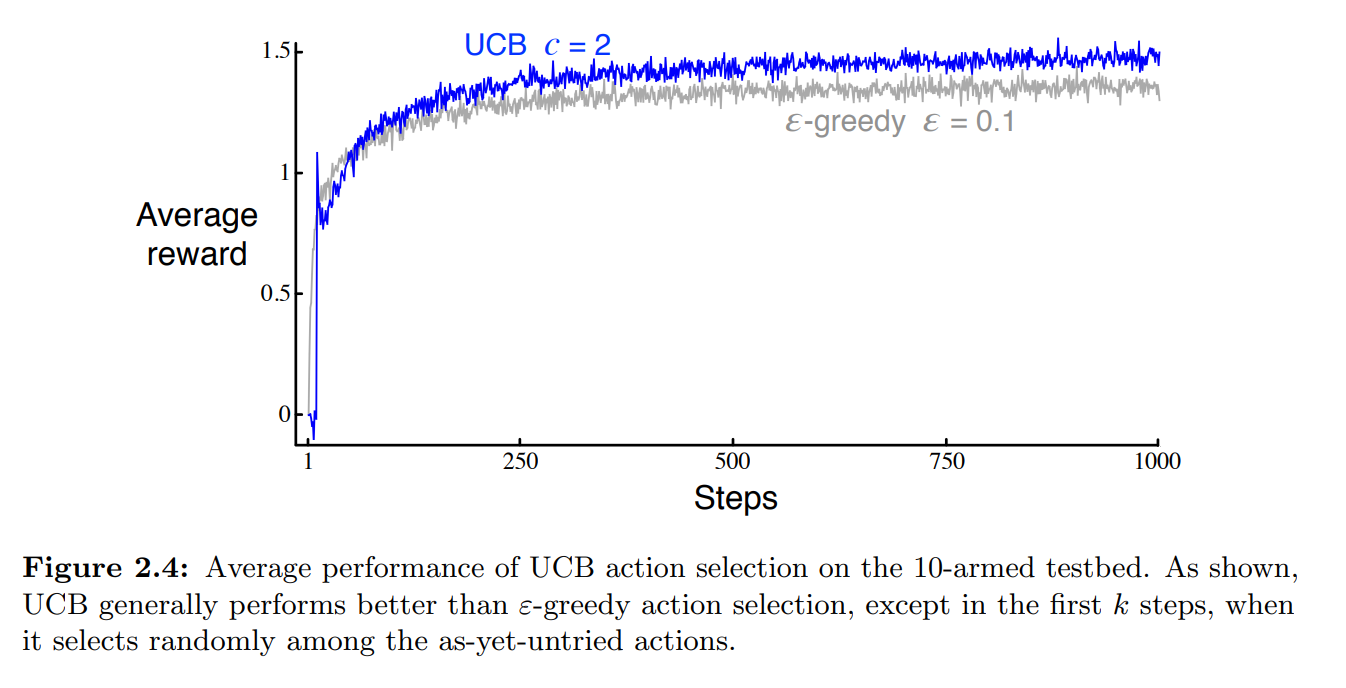
\includegraphics[scale=0.3]{./UCB_graph.png}

\subsubsection{Exercises}
\textit{Exercise 2.8}: \textit{UCB Spikes} In Figure 2.4 the UCB algorithm shows a distinct spike
in performance on the 11th step. Why is this? Note that for your answer to be fully
satisfactory it must explain both why the reward increases on the 11th step and why it
decreases on the subsequent steps. Hint: If \(c = 1\), then the spike is less prominent. 

After 10 timesteps the UCB algorithm has explored all 10 actions as, until they are selected,
their upper confidence bound is infinite (as \(N_t(a) = 0\)) as so it guarenteed to be selected once in
the first 10 actions. At this point the agent has one sample to assess the expected value of each
arm and the same confidence/uncertainty in each action. With the same \(c\) for every action, it is likely to pick the action
with highest return from first sample, which will likely give it an similarly large reward, creating
the spike. Now, the UCB for that action will decrease and the agent will
select another, less valuable action, causing the decrease in performance at the next timestep.




% --------------------------------------------------- SUBSECTION ------------------------------------------------
\subsection{Gradient Bandit Algorithms}
\begin{itemize}
\item Gradient bandit algorithms are a class of algorithms that use the gradient of the action-value function to select actions.
\item They are particularly useful in problems where the action space is continuous or large.
\item Gradient bandit algorithms maintain a preference for each action, which is updated based on the received rewards.
\item The action selection is based on a softmax function of the preferences, which allows for exploration and exploitation.
\item The preferences are updated using a gradient \textit{ascent} approach, where the update is proportional to the received reward and the difference between the action's preference and the average preference.
\item See the official book for the proofs of the equations.
\end{itemize}

\begin{equation}
    P(a) = \frac{e^{H(a)}}{\sum_{b=1}^{k} e^{H(b)}} = \pi_t(a)
\end{equation}

for \(k\) actions available, and $\pi_t(a)$ is the probability of selecting action \(a\) at time \(t\).

The preference for action \(a\) is denoted by \(H(a)\) is given by:
\begin{equation}
    H(a) \leftarrow H(a) + \alpha [R - \bar{R}] \cdot \frac{\partial P(a)}{\partial H(a)}
\end{equation}

where \(\bar{R}\) is the average reward of received up to but not including time \(t\), which serves as the \textbf{baseline}.

The baseline improves the performance significantly by adapting to the reward distribution shift by averaging the past rewards. 




% ---------------------------------------------------- SUBSECTION ------------------------------------------------
\subsection{Associative Search}

\begin{itemize}
\item So far, all the methods discussed has the learner's goal is to:
\subitem 
\begin{itemize}
    \item find the single best action if the task is stationary (reward probabilities don't change) or 
    \item to track the best action if the task is nonstationary (reward probabilities change over time). Note that it does NOT have knowledge about the changing state/situation and how they are relevant to action selection. 
    A situation can change suddenly, and it will have to relearn the best action. It doesn't associate the change with a new \textbf{type} of situation it needs to recognize; it just recognizes that the \textbf{effectiveness} of its actions has changed.
    \item There is no need to associate different actions with different situations.
\end{itemize}
\item However, in RL, there are many situations/environments with different best actions. 
\item The goal then is to learn a \textbf{poliicy} that \textit{maps states to actions} rather than just a single action.
\item In \textbf{associative search / contextual bandits}, the agent is given a set of actions and a set of contexts/clues. The agent must learn to select the best action for each context.
\item Associative tasks are intermediate between the \(n\)-armed bandit problem and the full RL problem:  They are like
the full RL problem in that they involve learning a policy, but they are also like our version of the \(k\)-armed bandit problem in that each action affects only the \textit{immediate} reward. 
If actions are allowed to affect the \textit{next situation} as well as the reward, then we have the full RL problem.
\end{itemize}



\subsubsection{Exercises}
\QuestionAnswer{
Suppose you face a 2-armed bandit task whose true action values change
randomly from time step to time step. Specifically, suppose that, for any time step,
the true values of actions 1 and 2 are respectively 10 and 20 with probability 0.5 (case
A), and 90 and 80 with probability 0.5 (case B). If you are not able to tell which case
you face at any step, what is the best expected reward you can achieve and how should
you behave to achieve it? Now suppose that on each step you are told whether you are
facing case A or case B (although you still don't know the true action values). This is an
associative search task. What is the best expected reward you can achieve in this task,
and how should you behave to achieve it?
}
{
If we select the actions at random, the expected reward is:
\begin{equation}
    E[R] = \frac{1}{2} \cdot E[R[A]] + \frac{1}{2} \cdot E[R[B]] = \frac{1}{2} (\cdot 10 + \frac{1}{2} \cdot 20) + \frac{1}{2} (\cdot 90 + \frac{1}{2} \cdot 80) = \frac{1}{2} (15 + 85) = 50
\end{equation}

In the associative search task, after a while, we will find out the best action for each situation. Then, we should keep picking that action for that situation, and the expected reward is:
\begin{equation}
    E[R] =  \cdot E[R[A]] + \cdot E[R[B]] =  (\frac{1}{2} \cdot 20) + (\frac{1}{2} \cdot 90) = (10 + 45) = 55.0
\end{equation}

}
